\documentclass[12pt,a4paper]{article}

% --- 1. CONFIGURACIÓN DE PÁGINA ---
\usepackage[left=2.54cm, right=2.54cm, top=2.54cm, bottom=2.54cm]{geometry}
\setlength{\headheight}{15pt}
\addtolength{\topmargin}{-2.5pt}

% --- 2. IDIOMA Y FUENTES ---
\usepackage{times}
\usepackage[utf8]{inputenc}
\usepackage[T1]{fontenc}
\usepackage[spanish, es-tabla]{babel}
\usepackage{csquotes}

% --- 3. INTERLINEADO Y SANGRÍA (APA 7) ---
\usepackage{setspace}
\doublespacing % Establece interlineado doble en todo el documento
\setlength{\parindent}{1.27cm} % Sangría de primera línea (Estándar APA es 0.5 pulgadas)

% --- 4. DISEÑO Y GRÁFICOS ---
\usepackage{caratula/caratula}
\usepackage{graphicx}
\graphicspath{{img/}}
\usepackage{pdflscape}
\usepackage{caption}
\usepackage{float}

\usepackage{amssymb}

% --- 5. TABLAS ---
\usepackage{booktabs}
\usepackage{array}
\usepackage{multirow}

% --- 6. ENCABEZADOS Y PIES ---
\usepackage{fancyhdr}
\usepackage{xcolor} 
\definecolor{gris_encabezado}{gray}{0.45}

% --- CONFIGURACIÓN DEL ÍNDICE ---
\usepackage{tocloft}
\addto\captionsspanish{
  \renewcommand{\contentsname}{Índice}
}
\renewcommand{\cfttoctitlefont}{\hfill\Large\bfseries}
\renewcommand{\cftaftertoctitle}{\hfill}
\renewcommand{\cftsecdotsep}{\cftdotsep}
\renewcommand{\cftsecfont}{\normalfont}
\renewcommand{\cftsecpagefont}{\normalfont}

\pagestyle{fancy}
\fancyhf{}
\renewcommand{\headrulewidth}{0pt}
\fancyhead[L]{\textcolor{gris_encabezado}{\small Aulla, Becerra , Millan \& Quinto}}
\fancyfoot[C]{\thepage}

\makeatletter
\fancypagestyle{lscape}{%
    \fancyhf{}%
    \fancyhead[L]{\textcolor{gris_encabezado}{\small Aulla, Becerra , Millan \& Quinto}}%
    \fancyfoot[C]{\thepage}%
    \renewcommand{\headrulewidth}{0pt}%
    \setlength{\footskip}{15pt}%
}
\makeatother

% --- 7. CÓDIGO FUENTE ---
\usepackage{listings}
\definecolor{codegreen}{rgb}{0,0.6,0}
\definecolor{codepurple}{rgb}{0.58,0,0.82}
\definecolor{backcolour}{rgb}{0.95,0.95,0.92}

\lstset{
    backgroundcolor=\color{backcolour},   
    commentstyle=\color{codegreen},
    keywordstyle=\color{blue},
    numberstyle=\tiny\color{gray},
    stringstyle=\color{codepurple},
    basicstyle=\ttfamily\footnotesize,
    breaklines=true,                 
    captionpos=b,                    
    numbers=left,                    
    frame=single,
    xleftmargin=1.5em
}

% --- 8. BIBLIOGRAFÍA ---
\usepackage[style=apa, backend=biber]{biblatex}
\addbibresource{referencias.bib}

% --- 9. DATOS ---
\titulo{Sistema de Registro Automatizado de Facturas mediante Inteligencia Artificial para la Prevención de Pérdida de Información en Almacenes Clínicos}
\alumnos{Aulla Gonzales, Jacson Michael \\ Becerra Sánchez, Guillermo Anibal \\ Millan Pariona, Mauricio Leandro  \\ Quinto Zapana, Gean Franco}
\curso{Innovación y Transformación Digital}
\docente{Mg. Anita Condo López}
\fecha{2026}

% --- CONFIGURACIÓN DE TÍTULOS ---
\usepackage{titlesec}

\usepackage{enumitem}

%\titleformat{\section}
%  {\normalfont\Large\bfseries}{}{0pt}{}

\begin{document}

\thispagestyle{empty}
\imprimircaratula
\clearpage


\begin{center}
    \vspace*{3cm}
    \normalsize \textbf{DEDICATORIA}
    \vspace{6cm}
\end{center}
\hspace{7.9cm}
\begin{minipage}{\dimexpr\textwidth-8cm}
    \textcolor{gray}{
        Le dedicamos este trabajo a nuestros familiares, amigos y compañeros,
        quienes nos han ayudado a alcanzar nuestros objetivos, apoyándonos y
        aconsejándonos en circunstancias poco favorables.
    }
\end{minipage}

\newpage

\begin{center}
    \vspace*{3cm}
    \normalsize \textbf{AGRADECIMIENTOS}
    \vspace{6cm}
\end{center}
\hspace{7.9cm}
\begin{minipage}{\dimexpr\textwidth-8cm}
    \textcolor{gray}{
        Expresamos nuestro sincero agradecimiento a nuestra docente guía, \textbf{Anita Condo López}, por su constante apoyo, orientación y dedicación durante el desarrollo de este proyecto.
    }
\end{minipage}

\newpage



% Reiniciamos numeración
\pagenumbering{arabic}
\setcounter{page}{1}

% Los índices suelen ir con interlineado sencillo para que no ocupen demasiadas hojas
\begin{singlespace}
    \tableofcontents \newpage
    %\listoffigures \newpage
    %\listoftables \newpage
\end{singlespace}

% --- CONTENIDO ---


\section*{\centering Introducción}
\addcontentsline{toc}{section}{Introducción}

Actualmente, la eficiencia de un laboratorio clínico no solo depende de la calidad de sus análisis, sino también de una gestión inteligente de sus recursos. Para el laboratorio Sermedsa E.I.R.L., el control de los reactivos es una prioridad, ya que de ello depende la continuidad de sus servicios y la seguridad analítica. En ese sentido, la empresa se encuentra en un proceso de modernización, buscando dejar atrás los métodos tradicionales de registro para adoptar soluciones digitales que centralicen su Información de inventarios.

Sin embargo, uno de los mayores desafíos detectados en la operatividad diaria es el ingreso de mercadería. Actualmente, cuando se reciben nuevos insumos, la información contenida en las facturas y boletas físicas debe ser procesada manualmente. Este método no solo consume tiempo valioso del personal, sino que genera un riesgo elevado de errores de transcripción y el peligro constante de que los documentos físicos se traspapelen antes de ser registrados correctamente en la base de datos, lo que afecta la precisión del stock real.

Para resolver esta problemática, el presente proyecto propone la implementación de un Módulo de Registro Automatizado mediante Inteligencia Artificial. La solución consiste en integrar una tecnología capaz de procesar imágenes de los comprobantes de pago y, mediante algoritmos de aprendizaje, identificar y extraer automáticamente los datos más importantes del documento para ingresarlos al sistema. De esta manera, se busca que la IA realice el trabajo de lectura y clasificación de datos, permitiendo que el personal solo tenga que validar la información.

Con esta innovación, Sermedsa busca dar un salto cualitativo en su gestión interna, logrando que el proceso de abastecimiento sea mucho más rápido, seguro y libre de papeles. El objetivo final es asegurar que toda la información crítica de los reactivos esté disponible de forma digital desde el momento en que ingresan al laboratorio, eliminando las brechas manuales que retrasan la operación.

\setcounter{section}{0}
\section{Descripción de la Empresa}

\subsection{Rubro del Negocio}

Sermedsa E.I.R.L. pertenece al sector de la salud y servicios médicos, operando específicamente en el rubro de los análisis de laboratorio clínico. Su actividad principal se centra en el procesamiento de muestras biológicas mediante el uso de reactivos químicos e insumos médicos especializados, brindando resultados precisos para el diagnóstico, prevención y tratamiento de diversas condiciones de salud.

\subsection{Misión y Visión}
\subsubsection{Misión}

Brindar servicios de análisis clínicos confiables, oportunos y de alta calidad, apoyando el diagnóstico médico y contribuyendo al bienestar de nuestros pacientes, a través de un manejo riguroso de nuestros procesos y recursos de laboratorio.

\subsubsection{Visión}
Ser reconocidos como un laboratorio clínico líder en la región, destacando por nuestra precisión diagnóstica, la modernización continua de nuestra infraestructura tecnológica y la eficiencia en la gestión de nuestros recursos operativos.

\subsection{Objetivos Estratégicos}

\begin{itemize}
    \item A corto plazo
          \begin{itemize}[label=-]
              \item Establecer una infraestructura digital centralizada que permita el control en tiempo real de los reactivos, eliminando progresivamente el uso de registros físicos y manuales en el almacén.
              \item Asegurar la trazabilidad de los insumos críticos mediante un sistema de alertas automáticas para el monitoreo de fechas de vencimiento.
          \end{itemize}
    \item A largo plazo
          \begin{itemize}[label=-]
              \item Lograr la automatización inteligente de la cadena de suministro mediante inteligencia artificial, permitiendo que el registro de entradas y el procesamiento de documentos de proveedores se realicen de forma autónoma.
          \end{itemize}
\end{itemize}

\section{Equipo Tecnológico}

Actualmente, la infraestructura tecnológica del laboratorio Sermedsa E.I.R.L. se compone de herramientas de ofimática convencionales y equipos de escritorio estándar, lo cual refleja un nivel de madurez digital básico que requiere ser actualizado para solucionar los cuellos de botella actuales.

\subsection{Software}
En cuanto a las herramientas lógicas y sistemas operativos en uso, la empresa emplea:
\begin{itemize}
    \item \textbf{Sistemas Operativos:} Windows 10 instalado en las estaciones de trabajo del área administrativa y recepción.
    \item \textbf{Ofimática y Gestión:} Microsoft Office, dependiendo casi en su totalidad de hojas de cálculo (Excel) para llevar el registro manual de los inventarios y reactivos.
    \item \textbf{Navegadores y Correo:} Uso de navegadores web estándar para la comunicación básica y recepción de cotizaciones de proveedores por correo electrónico.
\end{itemize}

\subsection{Hardware}
El equipamiento físico y de servidores con el que cuenta el laboratorio incluye:
\begin{itemize}
    \item \textbf{Estaciones de Trabajo:} Computadoras de escritorio estándar (procesadores Core i5 o equivalentes, 8GB de RAM) utilizadas por el personal administrativo y el jefe de laboratorio.
    \item \textbf{Periféricos de Digitalización:} Escáneres multifuncionales convencionales, los cuales actualmente se usan para copias, pero servirán como hardware base para capturar las imágenes de las facturas en el nuevo sistema.
    \item \textbf{Conectividad:} Red LAN local con acceso a internet de banda ancha. Actualmente, la empresa no cuenta con servidores físicos dedicados para bases de datos complejas.
\end{itemize}

\subsection{Soluciones}
Las implementaciones técnicas actuales se basan en soluciones aisladas y no integradas:
\begin{itemize}

    \item \textbf{Gestión Descentralizada:} No se cuenta con un sistema ERP (Planificación de Recursos Empresariales) ni un software centralizado para el manejo del almacén clínico.
    \item \textbf{Silos de Información:} El registro de ingresos de mercancía se almacena en archivos locales independientes, lo que imposibilita la visualización del stock en tiempo real y dificulta la auditoría de los comprobantes físicos.
\end{itemize}

\section{Informe de Madurez Digital}


El análisis de la situación actual del laboratorio Sermedsa E.I.R.L. evidencia un nivel de madurez digital básico. La organización opera principalmente mediante herramientas de ofimática convencional, como hojas de cálculo, y registros manuales, lo que limita la integración de la información y la automatización de sus procesos.

En el ámbito tecnológico, se identifica una fuerte dependencia de archivos locales y sistemas no integrados, lo cual genera silos de información y dificulta el acceso a datos en tiempo real. Asimismo, la ausencia de una plataforma centralizada impide una adecuada trazabilidad de los insumos y reduce la eficiencia en la gestión del inventario.

Desde el punto de vista operativo, los procesos actuales presentan múltiples ineficiencias, especialmente en el registro de ingresos de mercadería y el manejo de comprobantes físicos. Estas limitaciones incrementan el riesgo de errores humanos, pérdida de información crítica y retrasos en la actualización del stock.

En función de este diagnóstico, se identifican oportunidades de innovación de tipo incremental y radical. La innovación incremental se orienta a la digitalización y optimización de los procesos existentes, como la implementación de sistemas de control de inventario automatizados. Por otro lado, la innovación radical se refleja en la incorporación de tecnologías de inteligencia artificial para la extracción automática de datos desde comprobantes físicos, transformando completamente el flujo de trabajo tradicional.

Este análisis sustenta la necesidad de una transformación digital integral que permita mejorar la eficiencia operativa, reducir riesgos y garantizar una gestión de información más segura, precisa y escalable.


\section{Problemas de la Empresa}
\subsection{Problema 1}

Actualmente, el flujo de los reactivos en el laboratorio se maneja de forma analógica o mediante registro manuales aislados. Esta deficiencia operativa genera una falta de visibilidad sobre el stock real en tiempo real. al no existir una actualización automatica, el personal debe realizar verificaciones fisicas constantes para confirmar la disponibilidad de un insumo, lo que deriva en errores de inventario, compras de último minuto con sobrecostos y el riesgo de utilizar reactivos próximos a vencer por falta de alertas.

\subsection{Solución propuesta}

La estrategia de innovación consiste en el despliegue de una plataforma web (basada en la arquitectura propuesta previamente en Java/Spring Boot) que centralice el inventario. Esta solución permitirá automatizar el descuento de stock tras cada uso, generar reportes de consumo y establecer un sistema de notificaciones proactivas para el control de fechas de caducidad. Con esto, se logra una trazabilidad total de los insumos desde su ingreso hasta su descarte.

\subsection{Problema 2}

Este problema representa el mayor cuello de botella para la transformación digital de la empresa. Los proveedores entregan comprobantes físicos (facturas, boletas o guías de remisión) que deben ser almacenados y sus datos transcritos al sistema. Debido al alto volumen de trabajo, estos documentos suelen traspapelarse, dañarse o perderse antes de ser registrados. Esta pérdida de información física impide un control histórico de costos, dificulta la auditoría de compras y genera errores críticos al digitar manualmente datos complejos como números de lote.

\subsection{Solución propuesta}

Se propone el desarrollo de un módulo de extracción de datos automatizada mediante inteligencia artificial, lo cual constituye una innovación de tipo radical para la organización. A diferencia de un registro tradicional o una mejora incremental, esta solución introduce una tecnología disruptiva de aprendizaje automático que transforma por completo el flujo de trabajo: el personal captura una imagen del comprobante físico y la IA reconoce la estructura del documento, transcribiendo la información relevante de forma autónoma hacia el sistema. Con lo que, con este nuevo enfoque radical permitirá eliminar definitivamente la dependencia del papel y el error humano en la digitación, garantizando que el 100\% de las compras queden blindadas digitalmente desde el primer momento y redefiniendo la eficiencia operativa del almacén clínico.

\section{Propuesta Tecnológica}

\subsection{Roadmap Tecnológico Inicial}
Para superar las limitaciones actuales y lograr la automatización inteligente del almacén clínico, la implementación del proyecto se apoyará en la siguiente ruta de tecnologías clave:
\begin{itemize}
    \item \textbf{Inteligencia Artificial (Deep Learning):} Se utilizará para el desarrollo del módulo de lectura de facturas. Se justifica su uso porque es la tecnología idónea para el reconocimiento óptico (OCR avanzado) y la extracción autónoma de datos, permitiendo al sistema aprender la estructura de diferentes formatos de comprobantes y eliminando definitivamente el error humano en la digitación.
    \item \textbf{Cloud Computing (Nube):} La plataforma web de inventarios (basada en la arquitectura Java/Spring Boot) y su base de datos estarán alojadas en la nube. Se justifica esta decisión porque garantiza la escalabilidad del sistema, asegurando disponibilidad 24/7 de la información, protección contra pérdida de datos locales y facilidad técnica en caso de que Sermedsa abra nuevas sedes en el futuro.
\end{itemize}

\section{Plan de Gestión del Conocimiento}

Para asegurar la sostenibilidad de la innovación en Sermedsa E.I.R.L. y evitar la creación de "silos de información", se establece un flujo continuo de aprendizaje. Todo el conocimiento generado, como la configuración del modelo de Inteligencia Artificial, los manuales de usuario y las guías de resolución de errores, no recaerá en un solo individuo. Esta información será documentada y almacenada en un repositorio digital centralizado en la nube. De esta manera, se democratiza el acceso a la información, garantizando que el personal clínico y administrativo actual, así como futuros colaboradores, puedan operar el sistema de forma autónoma.

\section{Definición del Champion y Estrategia de Cambio}

Para liderar y asegurar el éxito de la implementación tecnológica, se ha designado como Champion a un miembro del equipo de desarrollo que labora internamente en Sermedsa E.I.R.L. Este perfil actúa como un ``Enlace Operativo'', ya que conoce a la perfección tanto los requerimientos técnicos del software como la cultura organizacional y las necesidades diarias del laboratorio.

Dado que el proyecto es de alcance local, la estrategia de relaciones se enfocará en gestionar la brecha tecnológica y generacional entre las nuevas herramientas de TI y el personal de salud tradicional, fuertemente habituado a los registros en papel. El Champion aprovechará su posición interna para actuar como un agente de confianza, liderando un acompañamiento empático y demostrando, mediante capacitaciones prácticas, que la Inteligencia Artificial es un aliado estratégico para reducir su carga administrativa, mitigando así cualquier resistencia al cambio.

\section{Solución del Proyecto}

\subsection{Alcance de la Tecnología}

El sistema se implementará como una aplicación web responsive, accesible de forma exclusiva desde cualquier navegador con conexión a internet. La plataforma priorizará la usabilidad y la experiencia del usuario para asegurar que las funciones principales (consultas, salidas y registros) sean intuitivas, contando con autenticación y roles básicos para un acceso controlado. Como límite de accesibilidad, el sistema no prevé un modo de funcionamiento sin conexión (offline) ni contempla el desarrollo de una aplicación móvil nativa para entornos Android o iOS, por lo que las operaciones requerirán conectividad permanente a la red.

En cuanto a la innovación principal del proyecto, el límite funcional radicará en el uso de modelos de Inteligencia Artificial (Deep Learning) aplicados exclusivamente para el reconocimiento óptico de caracteres (OCR) y la extracción autónoma de datos. Esta tecnología se utilizará de manera estricta para procesar las imágenes de las facturas y guías de remisión físicas, automatizando la digitalización de los insumos que ingresan al laboratorio.

A nivel de infraestructura, la arquitectura del sistema estará soportada íntegramente en la nube (Cloud Computing), utilizando herramientas como Java y el framework Spring Boot para la construcción lógica del sistema. Esta infraestructura permitirá que la información se concentre en un repositorio único que incluirá el catálogo de productos, lotes, fechas de caducidad y movimientos internos. Cada operación registrará los tiempos y los usuarios responsables para asegurar la trazabilidad, fortaleciendo la integridad y la calidad de la información.

Finalmente, el alcance analítico de la plataforma permitirá generar reportes de inventario vigente por producto, lote y ubicación, presentando indicadores clave como el stock mínimo y variaciones recientes para respaldar decisiones operativas. Sin embargo, el sistema gestionará estrictamente el inventario de un único almacén, por lo que no contemplará transferencias intersede ni reportes centralizados multisucursales.

\subsection{Flujo de solución}

El flujo de solución, define la secuencia de operaciones tecnológicas que transforman un documento físico en información estructurada dentro del sistema. En esta propuesta, el proceso automatizado inicia en la interfaz de "Registro de Compra", donde el empleado o gerente de almacén recibe la mercadería y captura o sube una imagen del comprobante físico (factura, boleta o guía de remisión) a la plataforma web.

A continuación, la imagen es enviada al módulo de Inteligencia Artificial, el cual procesa el documento mediante técnicas de reconocimiento óptico (OCR) y aprendizaje profundo (Deep Learning) para identificar y extraer de forma autónoma los datos más relevantes, tales como el nombre del proveedor, descripción de los reactivos, cantidades, número de lote y fechas de vencimiento.

Una vez que la Inteligencia Artificial finaliza la extracción, el sistema pre-llena el formulario en la pantalla del usuario. En esta etapa final, el empleado revisa y aprueba la información extraída. Tras la validación humana, el sistema actualiza el stock en la base de datos de manera centralizada, finalizando el proceso de abastecimiento de forma segura y sin digitación manual.

\subsubsection{Diagrama de Casos de Uso}

\begin{figure}[H]
    \centering
    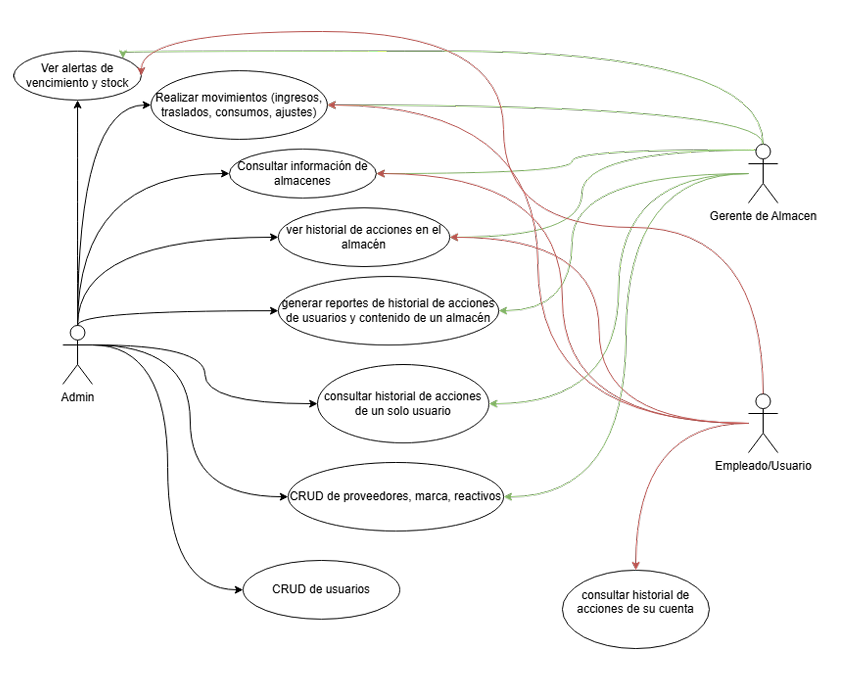
\includegraphics[width=1\textwidth]{CasoUso.png}
    \caption{Diagrama de caso de uso del proyecto}
    \label{fig:caso_uso}
\end{figure}

\subsubsection{Diagrama de Secuencia}

\begin{figure}[H]
    \centering
    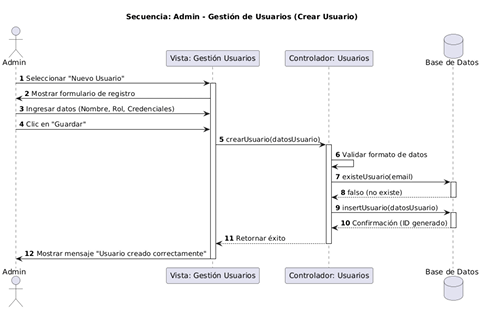
\includegraphics[width=0.8\textwidth]{Administrador.png}
    \caption{Diagrama de Secuencia del administrador}
    \label{fig:seq_admin}
\end{figure}

\begin{figure}[H]
    \centering
    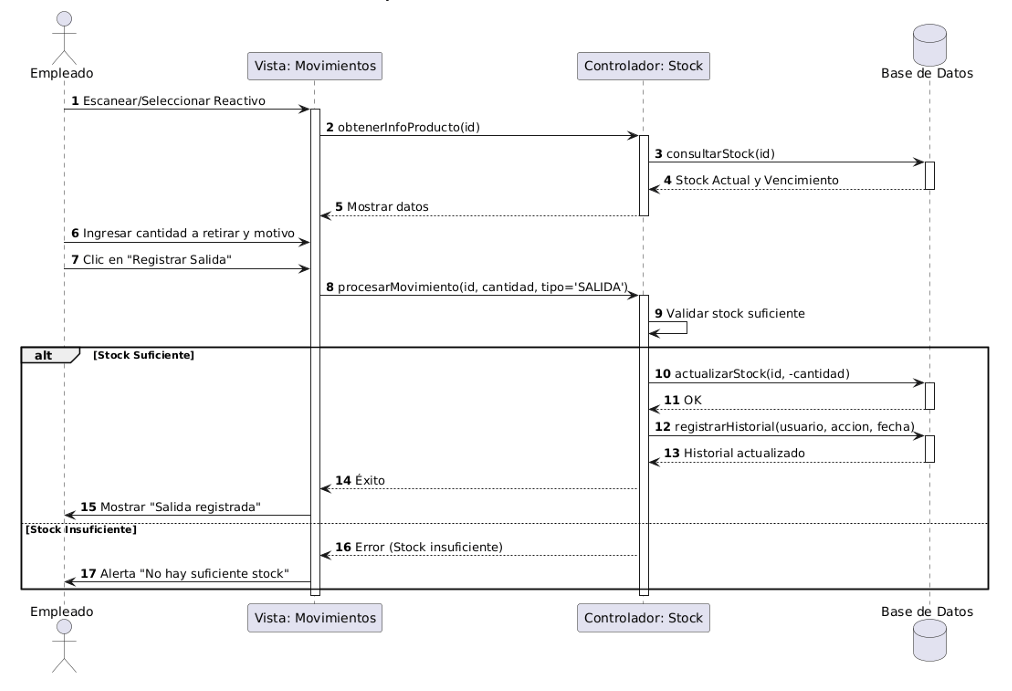
\includegraphics[width=0.8\textwidth]{Empleado.png}
    \caption{Diagrama de Secuencia del Empleado}
    \label{fig:seq_empleado}
\end{figure}

\begin{figure}[H]
    \centering
    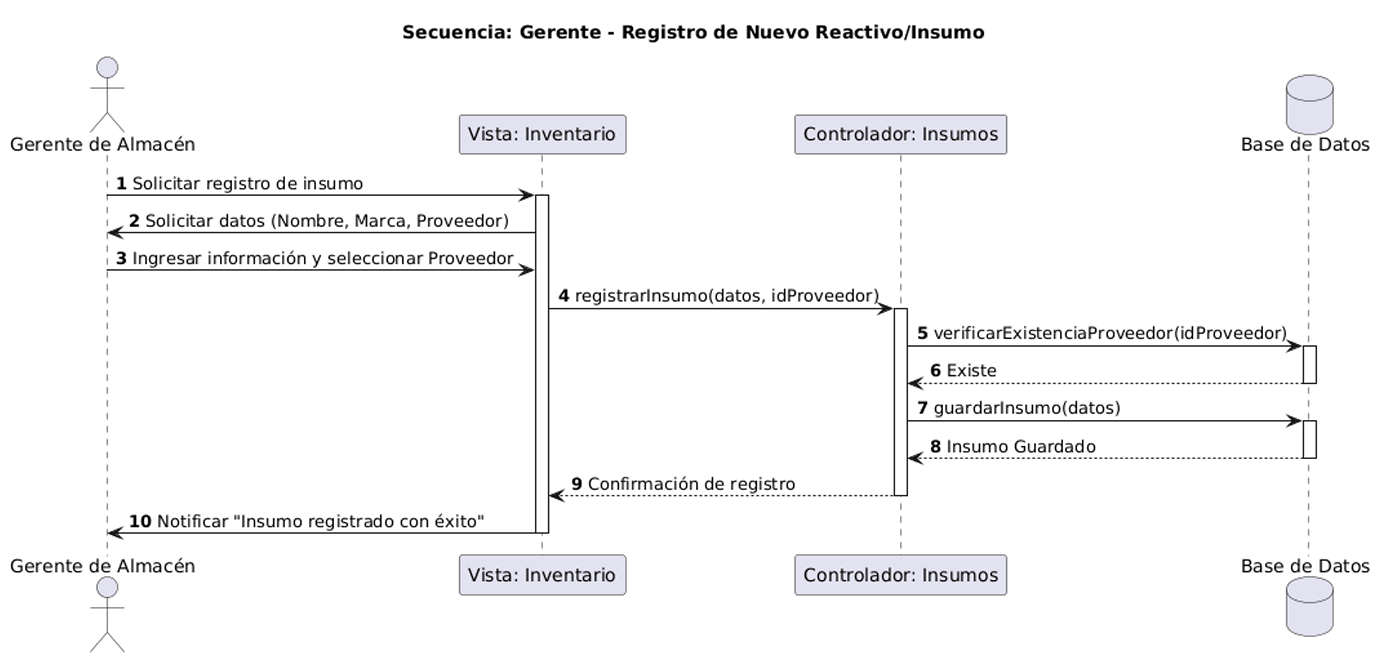
\includegraphics[width=0.8\textwidth]{Gerente.png}
    \caption{Diagrama de Secuencia del Gerente de Almacén}
    \label{fig:seq_gerente}
\end{figure}

\subsection{Desarrollo del Prototipo Inicial}

Bajo los principios de la metodología Lean Startup, los wireframes presentados a continuación no solo representan un diseño visual, sino que constituyen el Producto Mínimo Viable (PMV) del sistema. La estructuración de las interfaces se apoyó en la metodología Design Thinking para empatizar con el usuario final, centrando el diseño en la usabilidad, con una interfaz limpia y navegación intuitiva. El objetivo de este PMV es materializar la funcionalidad de la Inteligencia Artificial con la mínima inversión de desarrollo, permitiendo iniciar el circuito de aprendizaje validado (Construir-Medir-Aprender) con el personal del laboratorio antes de la fase de codificación intensiva.

\begin{figure}[H]
    \centering
    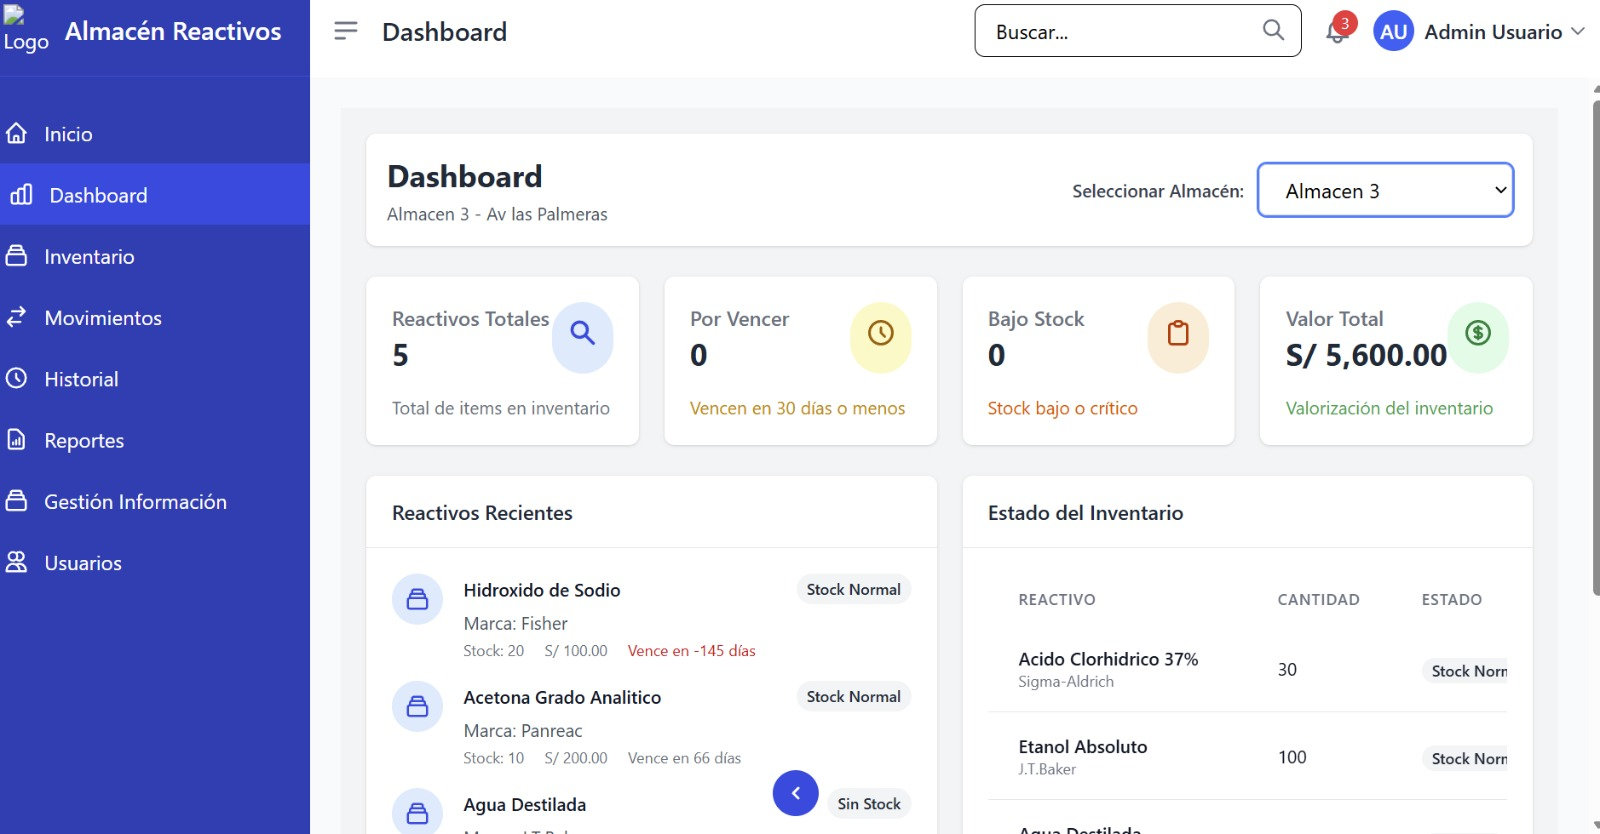
\includegraphics[width=1\textwidth]{ProtoDashboard.jpeg}
    \caption{PMV - Interfaz del Dashboard (Panel de Control Principal)}
    \label{fig:proto_dashboard}
\end{figure}

\begin{figure}[H]
    \centering
    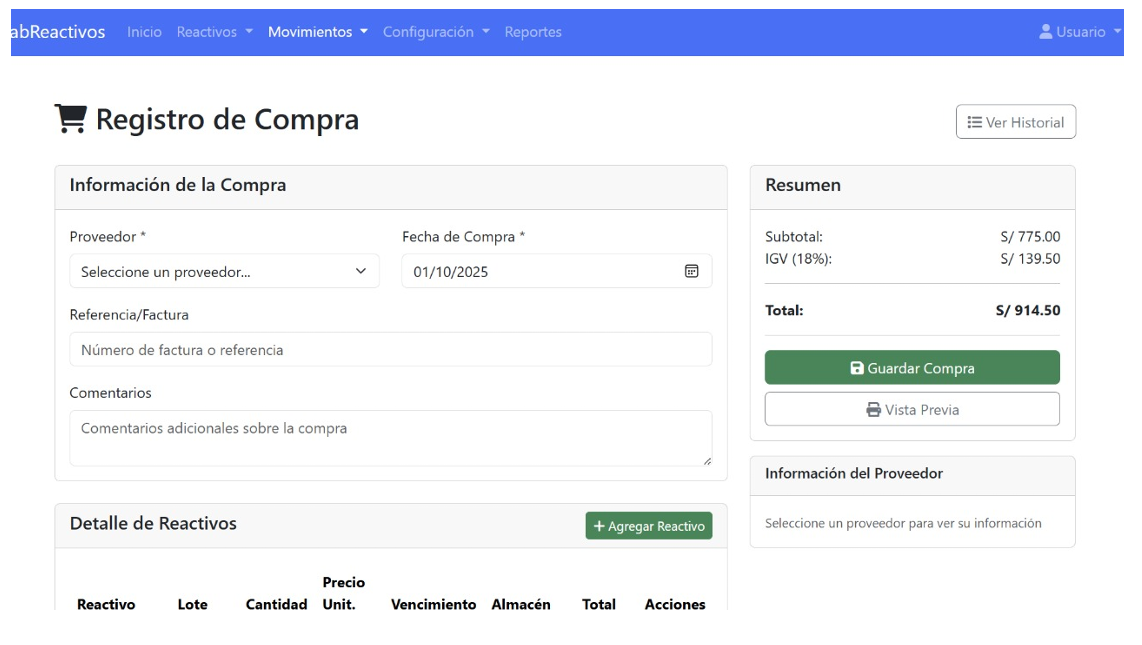
\includegraphics[width=1\textwidth]{ProtoCompra.png}
    \caption{PMV - Interfaz de Registro Automatizado de Compras con integración de IA}
    \label{fig:proto_compra}
\end{figure}

\begin{figure}[H]
    \centering
    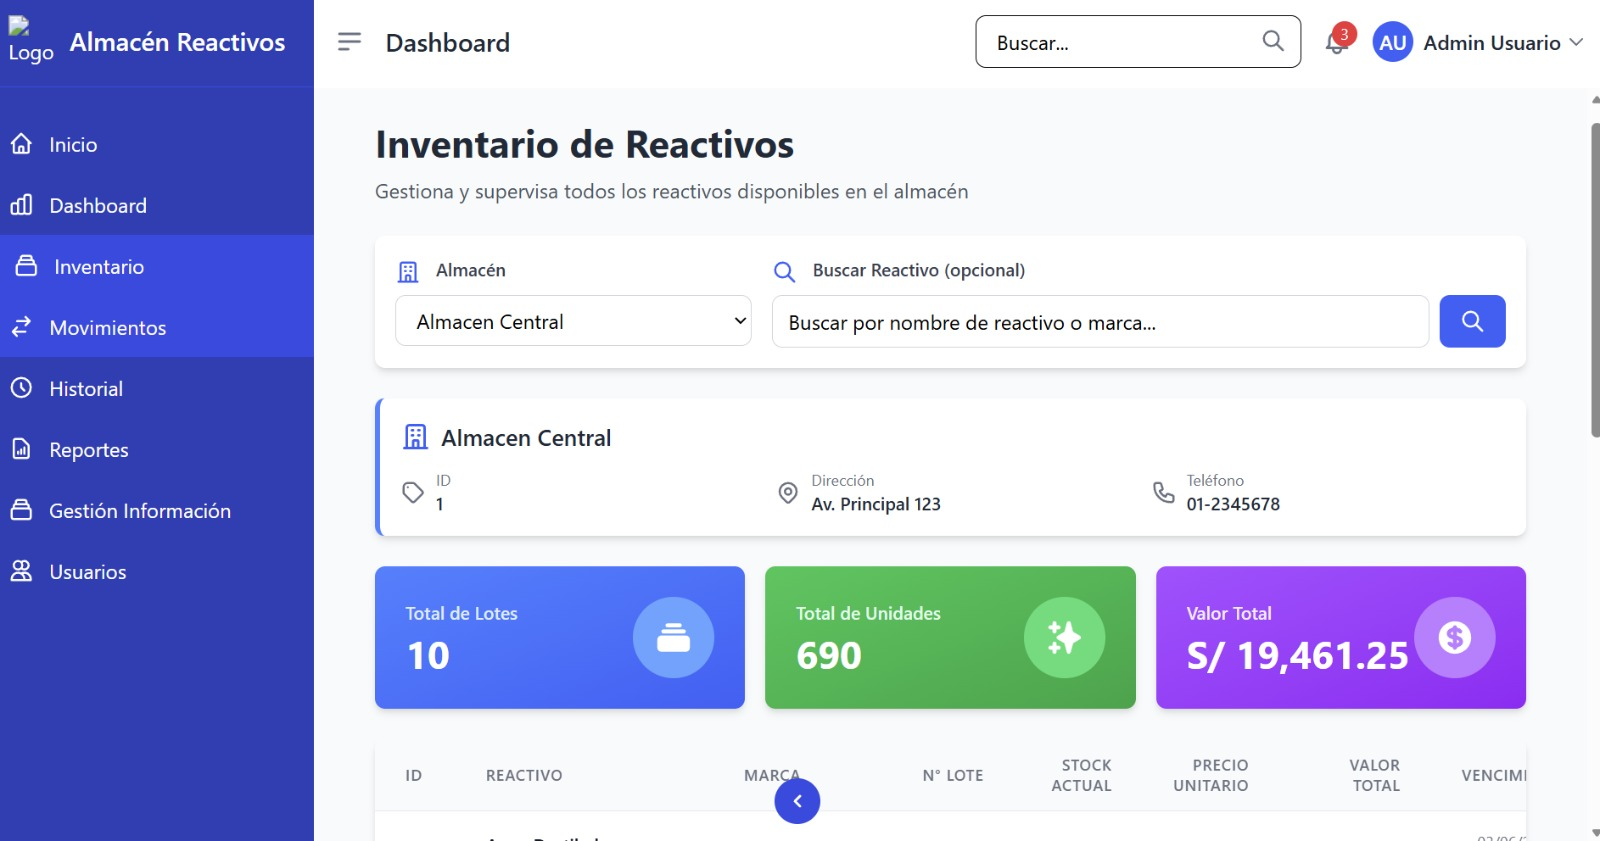
\includegraphics[width=1\textwidth]{ProtoInventario.jpeg}
    \caption{PMV - Interfaz del Inventario de Reactivos}
    \label{fig:proto_inventario}
\end{figure}

\section{Metodología Ágil}

\subsection{Titulo del proyecto}

Sistema de Registro Automatizado de Facturas Mediante Inteligencia Artificial para la Prevención de Pérdida de Información en Almacenes Clínicos

\subsection{Diseño de la metodología ágil}

Para el desarrollo de esta solución tecnológica, se ha adoptado el modelo de sinergia propuesto por Gartner. Este modelo estructura la innovación en tres ejes fundamentales: Design Thinking para empatizar y definir el problema del cliente, Lean Startup para experimentar y validar la solución mediante el PMV, y Agile para la ejecución y entrega continua de valor.

Bajo el eje de ejecución Agile, se ha adoptado un enfoque híbrido integrando Scrum y Kanban. Scrum proporciona una estructura iterativa e incremental mediante ciclos cortos de prueba y error (Sprints), lo cual es fundamental para el entrenamiento e integración del módulo de Inteligencia Artificial. Por su parte, Kanban se implementa como un sistema visual de desarrollo continuo para gestionar el flujo de trabajo del equipo de desarrollo, permitiendo identificar cuellos de botella en tiempo real y optimizar la eficiencia.

A nivel organizacional, el equipo actual se configura como un único equipo ágil. Sin embargo, proyectando el crecimiento a largo plazo del laboratorio hacia nuevas sucursales y previendo la necesidad de ampliar el departamento de TI, se establece como framework de escalamiento LeSS (Large-Scale Scrum). Bajo el principio fundamental de que ``Scrum a gran escala es Scrum'', este marco permite que múltiples equipos autogestionados trabajen juntos en la construcción del mismo producto. Si la empresa expande sus operaciones, el sistema escalará manteniendo una estructura plana y centrada en el cliente: los futuros equipos técnicos compartirán un único Product Owner (para mantener la visión del negocio centralizada) y un único Product Backlog, colaborando continuamente para entregar un incremento de software integrado sin necesidad de añadir capas burocráticas.

A nivel estratégico, la adopción del sistema se respalda en la metodología Lean Change Management. Dado que la transición de registros en papel hacia una automatización con IA generará un impacto directo en las rutinas del personal, este marco permite gestionar la resistencia al cambio basándose en la experimentación y la co-creación.

\subsubsection{Roles y Responsabilidades}

Dentro de nuestro equipo, los roles han sido asignados bajo los estándares del marco ágil para asegurar la entrega de valor:

\begin{itemize}
    \item \textbf{Product Owner}: Millan Pariona, Mauricio Leandro.
    \item \textbf{Scrum Master}: Aulla Gonzales, Jacson Michael.
    \item \textbf{Equipo de Desarrollo}: Becerra Sánchez, Guillermo Anibal y Quinto Zapana, Gean Franco.
\end{itemize}

\subsection{Planificación del Proyecto}
\subsubsection{Roadmap del proyecto}

La ruta estratégica de desarrollo se estructura en un ciclo de cuatro fases de entrega continua. En lugar de una planificación predictiva tradicional, estas fases representan los grandes hitos que el equipo abordará de manera iterativa, asegurando la integración progresiva de la Inteligencia Artificial:

\begin{itemize}
    \item \textbf{Fase 1: Estructuración y Prototipado.} Definición del Product Backlog inicial, diseño de la arquitectura en la nube (Cloud) y validación visual de interfaces mediante prototipos de baja y alta fidelidad.
    \item \textbf{Fase 2: Core del Sistema Web.} Construcción del modelo de datos relacional y desarrollo del Backend transaccional (Spring Boot) necesario para la gestión del inventario base y la seguridad del sistema.
    \item \textbf{Fase 3: Innovación y Automatización.} Esta fase concentra el esfuerzo en el entrenamiento del modelo de IA (OCR), la creación del endpoint de procesamiento de imágenes y su acoplamiento funcional con la interfaz de "Registro de Compra".
    \item \textbf{Fase 4: Pruebas y Despliegue.} Ejecución iterativa de pruebas unitarias y de vulnerabilidad, ajuste de la precisión de lectura de la IA y despliegue del sistema final en el entorno de producción.
\end{itemize}

\subsubsection{Cronograma de actividades y Rituales Ágiles}

La planificación temporal del proyecto se estructura a través de iteraciones cortas denominadas Sprints, cada una con una duración establecida de dos semanas. Aplicando el marco LeSS, el progreso iterativo e incremental se gestiona mediante los siguientes rituales colaborativos:

\begin{itemize}
    \item \textbf{Refinamiento (Backlog Refinement):} Evento colaborativo a mitad de la iteración para esclarecer el trabajo de futuros Sprints junto al cliente y los usuarios finales, liberando al Product Owner para enfocarse en la priorización estratégica.
    \item \textbf{Sprint Planning 1 y 2:} La planificación se divide en dos fases. En el Planning 1, el equipo selecciona las historias de usuario priorizadas que aportan más valor al negocio. En el Planning 2, los desarrolladores discuten y deciden las estrategias técnicas y de arquitectura para programar dichas historias.
    \item \textbf{Daily Scrum:} Reunión diaria de coordinación donde el equipo autogestionado se sincroniza operativamente frente al tablero visual.
    \item \textbf{Sprint Review:} Sesión compartida donde se evalúa el incremento de software funcional terminado y se decide qué aportará más valor en la siguiente iteración.
    \item \textbf{Retrospectiva General:} Inspección y adaptación del proceso de trabajo para explorar y remover obstáculos sistémicos u organizacionales, buscando la mejora continua.
\end{itemize}

\begin{figure}[H]
    \centering
    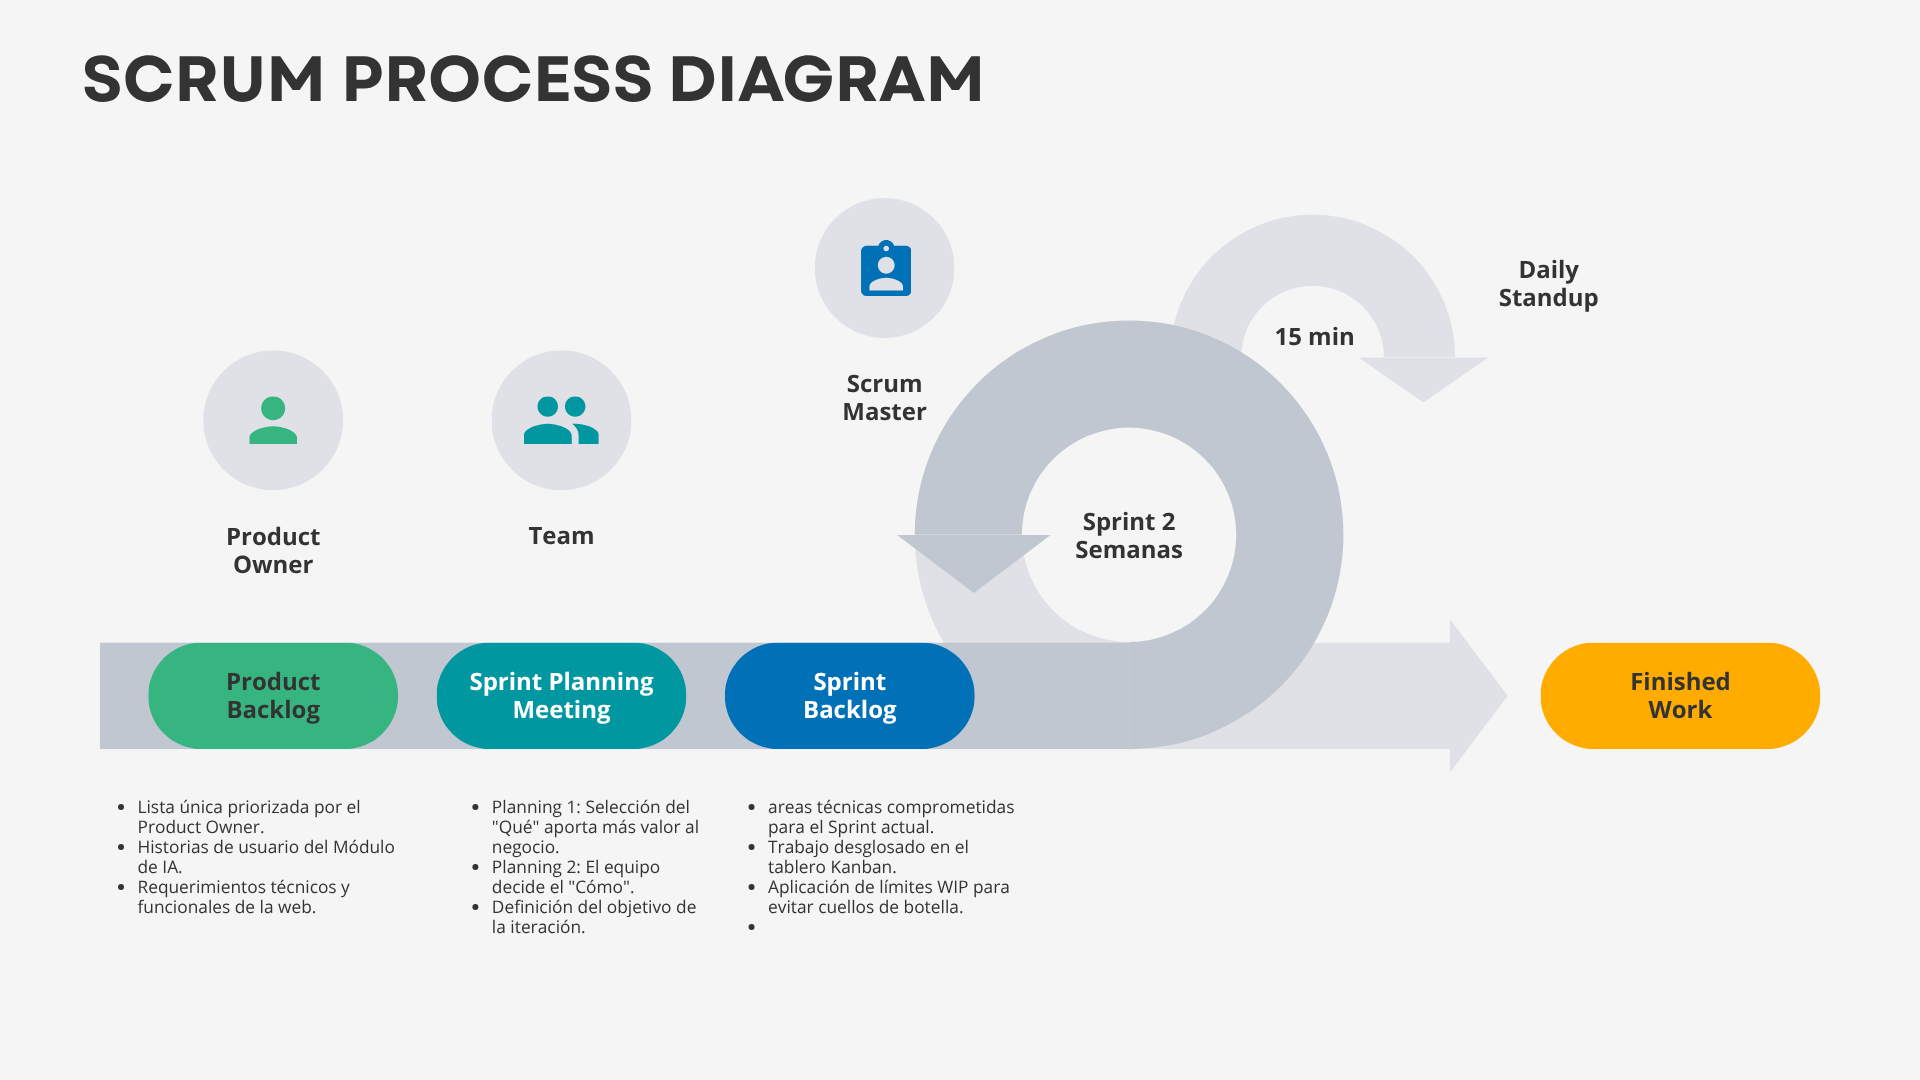
\includegraphics[width=0.9\textwidth]{Scrum.png}
    \caption{Esquema del ciclo iterativo Scrum para el proyecto}
    \label{fig:esquema_scrum}
\end{figure}

\subsubsection{Gestión Visual mediante Kanban}

Para complementar las iteraciones de Scrum y garantizar la transparencia del trabajo diario, el equipo emplea un tablero Kanban digital. La implementación de este marco se rige por los cinco principios fundamentales de la metodología: Visualización del flujo, Priorización de tareas, Mejora continua, Liderazgo en todos los niveles, y Calidad garantizada.

Bajo la filosofía central de "Stop starting, start finishing", las historias de usuario transitan visualmente por un flujo de estados claramente definido:

\begin{itemize}
    \item \textbf{To Do (Por Hacer):} Requerimientos priorizados en el Backlog y listos para iniciar.
    \item \textbf{In Progress (En Progreso):} Tareas que los desarrolladores (Guillermo y Gean) están codificando activamente.
    \item \textbf{Code Review / Testing (Revisión y Pruebas):} El código se revisa por pares y se ejecutan las pruebas unitarias. En esta fase se aplican estrictos Límites WIP (Work In Progress) para evitar la sobrecarga de los programadores, detectar cuellos de botella y mantener un flujo estable.
    \item \textbf{Done (Terminado):} La tarea cumple con la Definición de Hecho (Definition of Done) y está lista para el despliegue.
\end{itemize}

\begin{figure}[H]
    \centering
    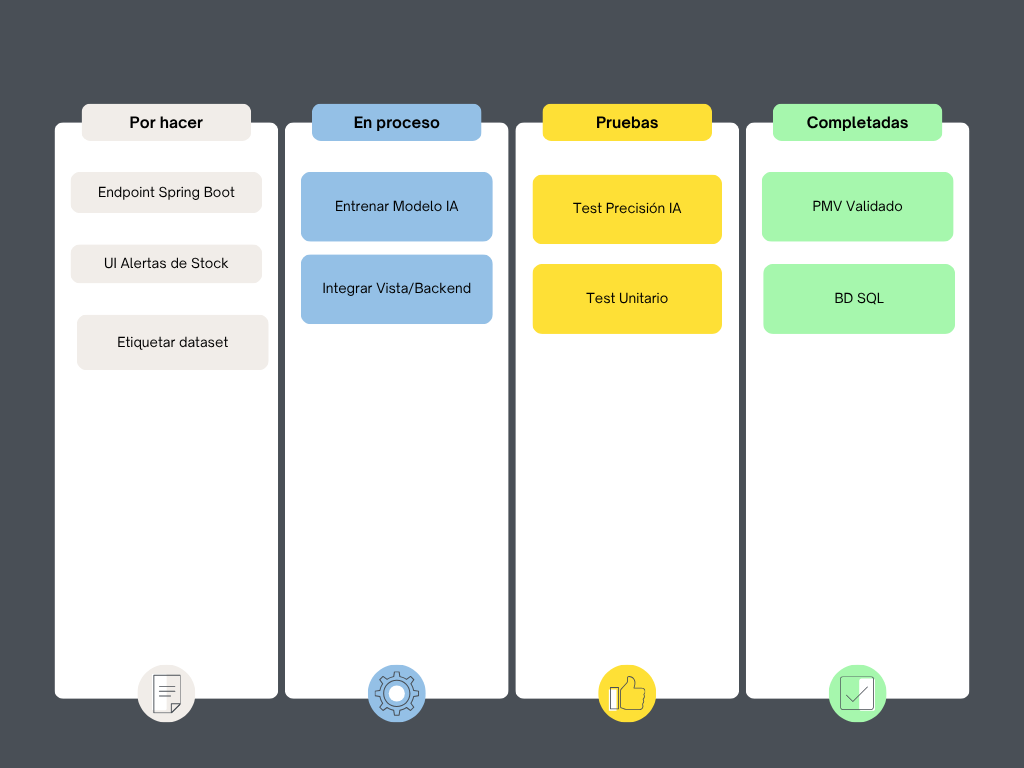
\includegraphics[width=1\textwidth]{Kanban.png}
    \caption{Tablero Kanban del equipo mostrando el flujo continuo, tareas técnicas y límites WIP}
    \label{fig:tablero_kanban}
\end{figure}

\section{Validación Inicial}

Continuando con el ciclo de la metodología Lean Startup, el Producto Mínimo Viable (PMV) —representado en esta etapa por los prototipos visuales interactivos— fue sometido a la fase de medición mediante pruebas de interacción directa con el personal de Sermedsa E.I.R.L..

\subsection{Pruebas preliminares y Retroalimentación}
Durante las sesiones de validación frente al monitor, el usuario evaluó la usabilidad general y la propuesta de interacción con el futuro sistema automatizado.
\begin{itemize}
    \item \textbf{Feedback obtenido:} Los usuarios reportaron que la navegación de la interfaz es fluida e intuitiva. Respecto a la innovación de reconocimiento óptico, validaron positivamente la propuesta, confirmando que delegar la transcripción de las facturas a la Inteligencia Artificial reducirá drásticamente su carga administrativa y mitigará el riesgo de cometer errores de digitación en los números de lote.
    \item \textbf{Aplicación de Lean Change Management:} Las sugerencias operativas obtenidas durante la sesión fueron registradas para ser incorporadas en el diseño final. Esto demuestra que fomentar la co-creación y hacer partícipe al usuario en la propuesta visual, antes de codificar la solución, facilita enormemente la adopción tecnológica y disminuye la resistencia al cambio.
    \item \textbf{Aprendizaje validado (Iterar o Pivotar):} Al confirmar la hipótesis central de que la automatización visualizada en el PMV soluciona un problema real y es bien recibida por el personal, se consolida un aprendizaje validado positivo. En consecuencia, la decisión estratégica del equipo es \textbf{Iterar} sobre la propuesta actual, dando inicio al desarrollo técnico (programación del Backend en Spring Boot y entrenamiento del modelo de IA) sin necesidad de pivotar hacia una funcionalidad distinta.
\end{itemize}

\begin{figure}[H]
    \centering
    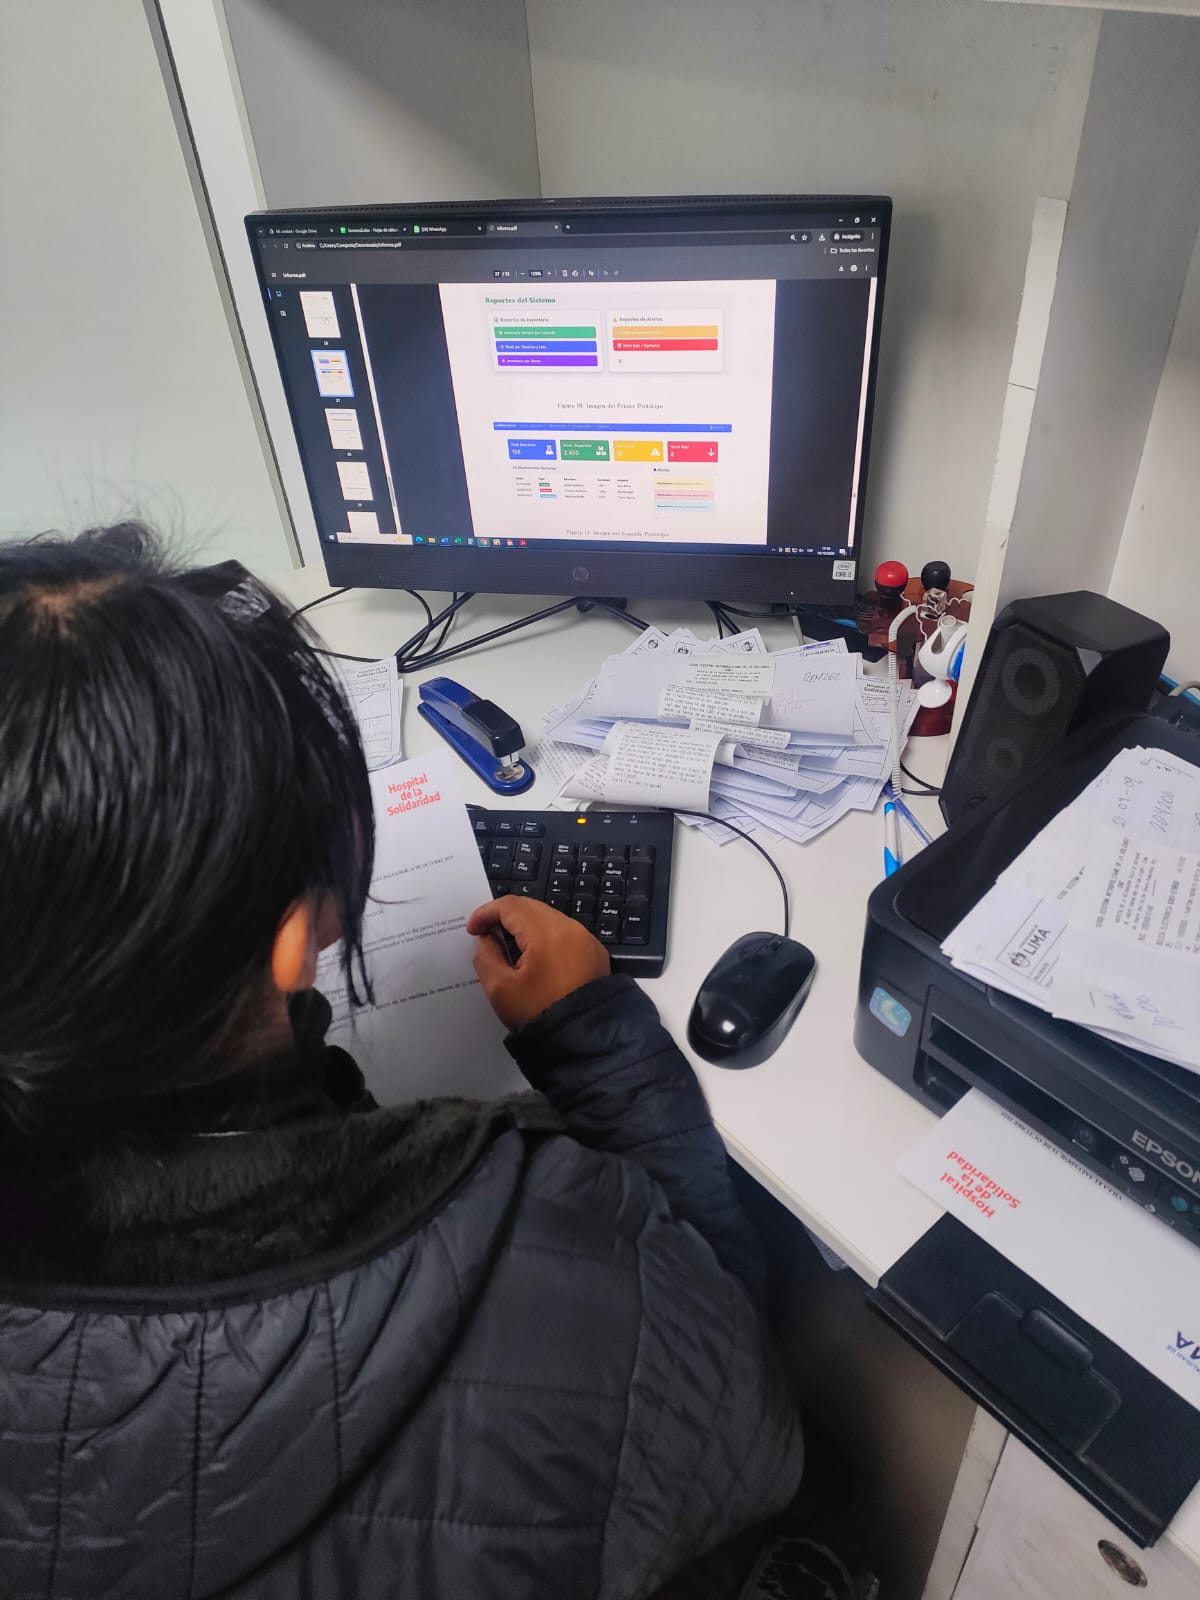
\includegraphics[width=0.5\textwidth]{evidencia1.jpg}
    \caption{Evidencia de validación visual del PMV con el usuario}
    \label{fig:evidencia_1}
\end{figure}

\begin{figure}[H]
    \centering
    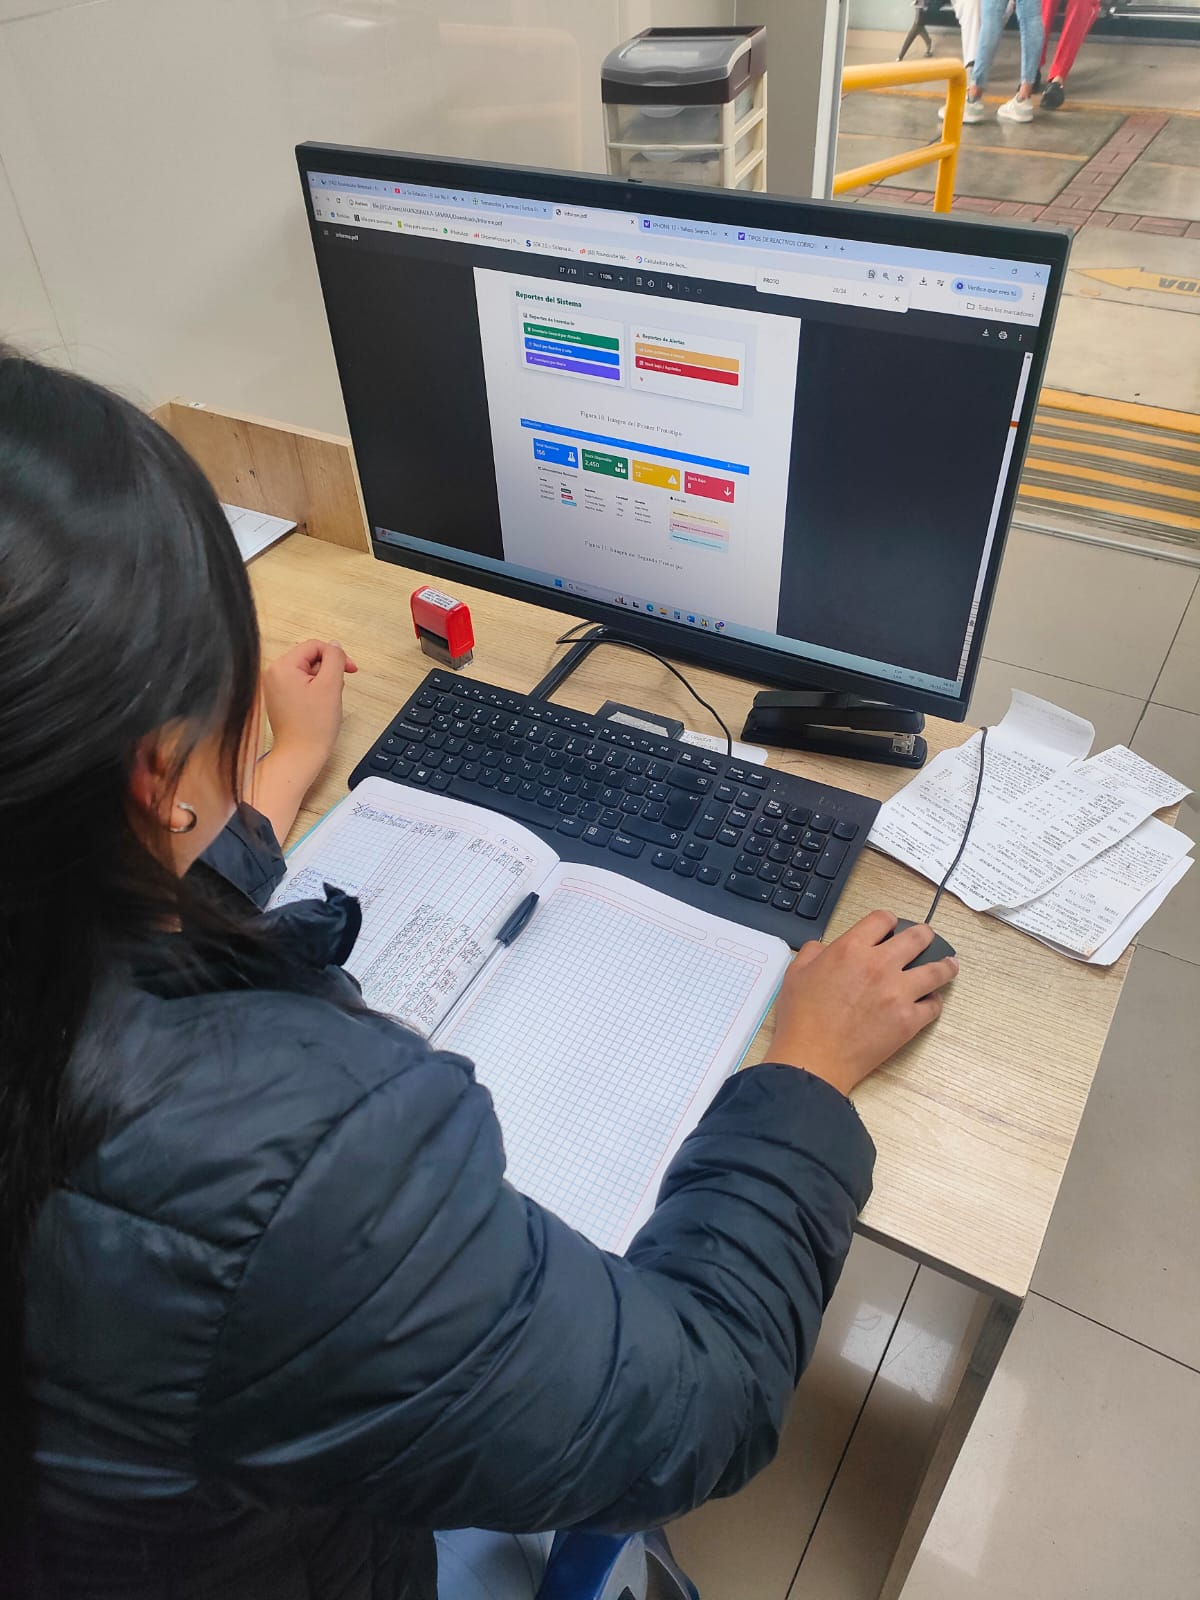
\includegraphics[width=0.5\textwidth]{evidencia2.jpg}
    \caption{Evidencia de validación visual del PMV con el usuario}
    \label{fig:evidencia_2}
\end{figure}

\begin{figure}[H]
    \centering
    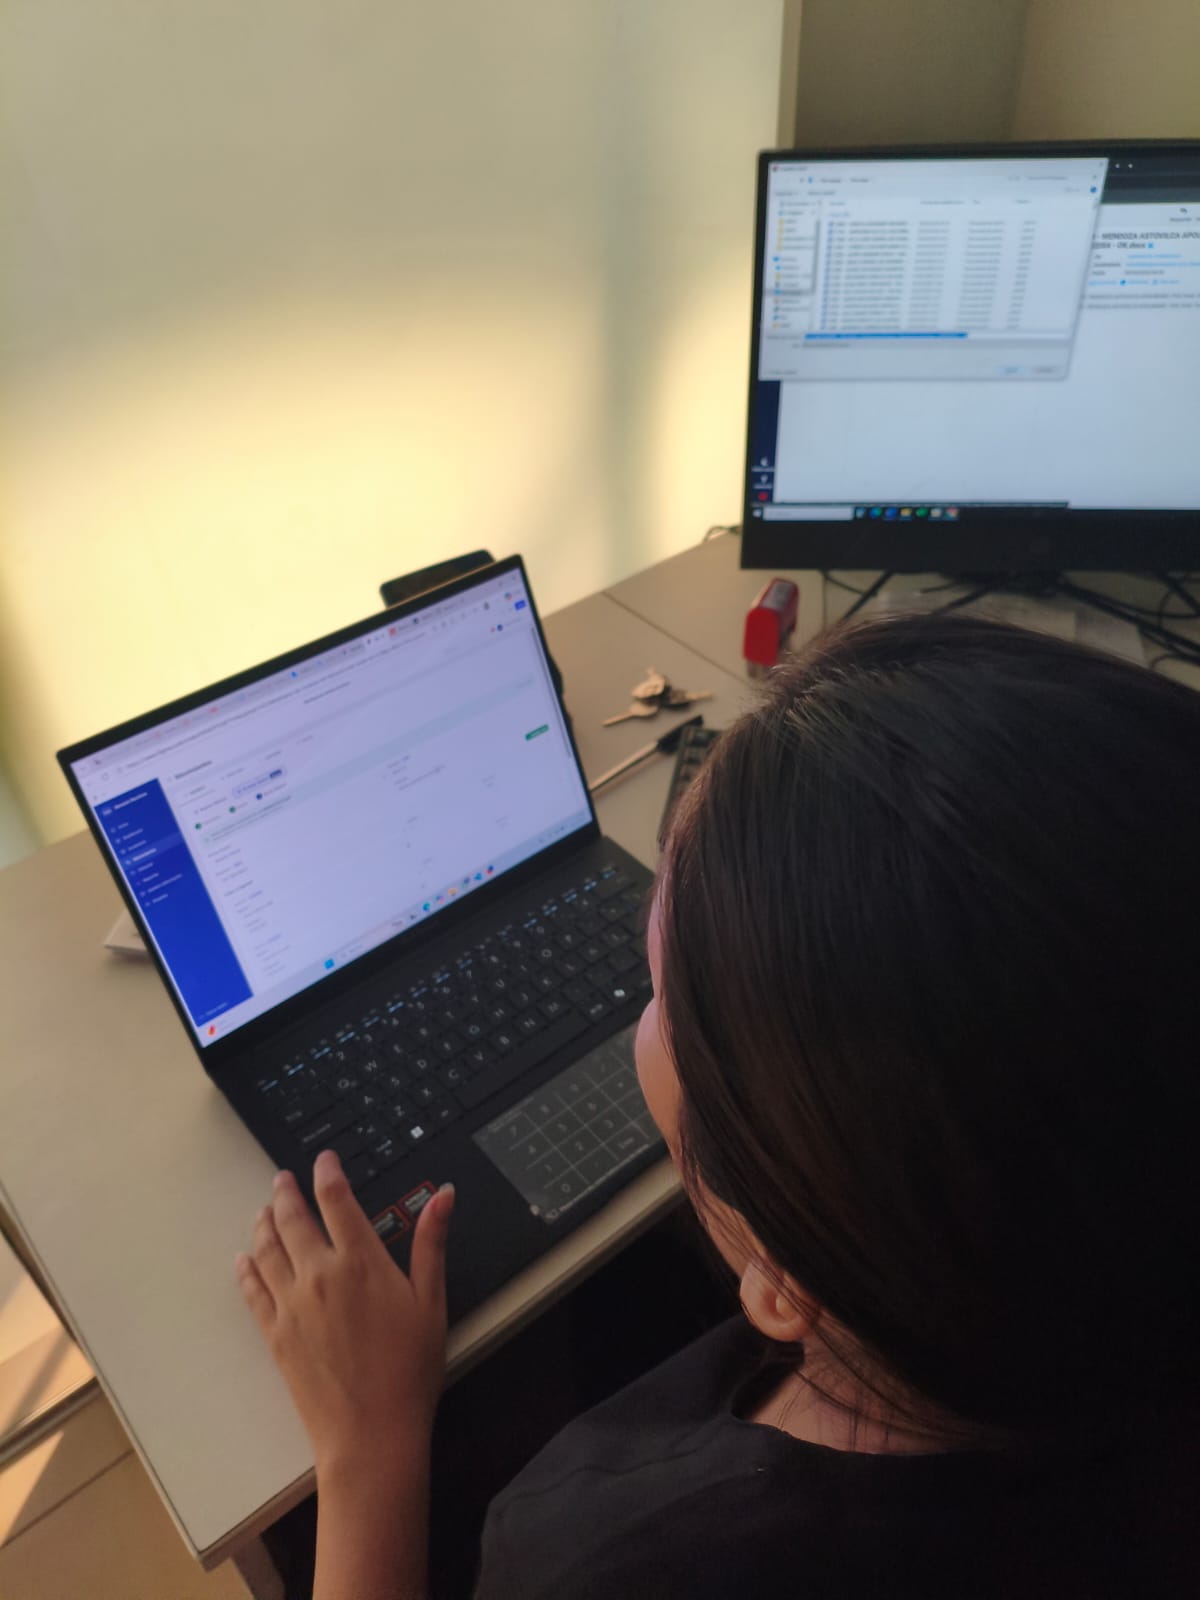
\includegraphics[width=0.5\textwidth]{evidencia3.jpeg}
    \caption{Evidencia de validación visual del PMV con el usuario}
    \label{fig:evidencia_3}
\end{figure}



\section{\textbf{ANEXO}}

\begin{figure}[H]
    \centering
    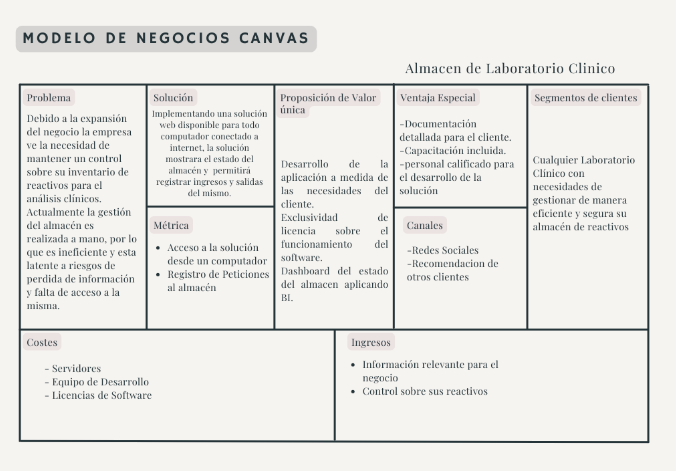
\includegraphics[width=1\textwidth]{Lean Canvas.png}
    \caption{Lean Canvas del proyecto}
    \label{fig:lean_canvas}
\end{figure}


\begin{table}[H]
    \centering
    \caption{Diagrama de Gantt del Proyecto (12 Semanas)}
    \label{tab:gantt_proyecto}
    \renewcommand{\arraystretch}{1.8}
    \resizebox{\linewidth}{!}{%
        \begin{tabular}{@{} l *{12}{c} @{}}
            \toprule
            \multirow{2}{*}{\textbf{Fases y Tareas del Proyecto}} & \multicolumn{12}{c}{\textbf{Semanas Operativas (Año 2026)}}                                                                                                                                                                                                                                                                                    \\
            \cmidrule(l){2-13}
                                                                  & \textbf{S5}                                                 & \textbf{S6}            & \textbf{S7}            & \textbf{S8}            & \textbf{S9}            & \textbf{S10}           & \textbf{S11}           & \textbf{S12}           & \textbf{S13}           & \textbf{S14}           & \textbf{S15}           & \textbf{S16}           \\
                                                                  & {\footnotesize 20 Abr}                                      & {\footnotesize 27 Abr} & {\footnotesize 04 May} & {\footnotesize 11 May} & {\footnotesize 18 May} & {\footnotesize 25 May} & {\footnotesize 01 Jun} & {\footnotesize 08 Jun} & {\footnotesize 15 Jun} & {\footnotesize 22 Jun} & {\footnotesize 29 Jun} & {\footnotesize 06 Jul} \\
            \midrule
            1. Reconocimiento de Arquitectura Actual              & $\blacksquare$                                              &                        &                        &                        &                        &                        &                        &                        &                        &                        &                        &                        \\
            2. Planeación y Selección                             &                                                             & $\blacksquare$         &                        &                        &                        &                        &                        &                        &                        &                        &                        &                        \\
            3. Diseño UI/UX                                       &                                                             &                        & $\blacksquare$         & $\blacksquare$         &                        &                        &                        &                        &                        &                        &                        &                        \\
            4. Arquitectura                                       &                                                             &                        &                        & $\blacksquare$         & $\blacksquare$         &                        &                        &                        &                        &                        &                        &                        \\
            5. Desarrollo de Backend                              &                                                             &                        &                        &                        &                        & $\blacksquare$         & $\blacksquare$         & $\blacksquare$         & $\blacksquare$         &                        &                        &                        \\
            6. Motor de Validación y Reglas                       &                                                             &                        &                        &                        &                        &                        &                        &                        & $\blacksquare$         & $\blacksquare$         &                        &                        \\
            7. Pruebas QA y Casos de Borde                        &                                                             &                        &                        &                        &                        &                        &                        &                        &                        &                        & $\blacksquare$         & $\blacksquare$         \\
            8. Despliegue y Capacitación                          &                                                             &                        &                        &                        &                        &                        &                        &                        &                        &                        &                        & $\blacksquare$         \\
            \bottomrule
        \end{tabular}%
    }
\end{table}


\end{document}